
\chapter{The soft-handover balancing problem \label{chap:07-Experimental-evaluation-the-SHO-alignment-problem}}

% First paragraph has no indentation.

\noindent In Chapter~\ref{chap:06-Experimental-evaluation-the-service-coverage-problem},
an application exploiting the advantages of faster evaluation methods
has been presented. Solving the service-coverage problem for real-world
networks capitalizes on the ability to tackle bigger problem instances.
Because of their size, such problems were previously unsolvable in
a feasible amount of time. This improved performance also allows solving
optimization problems with a higher degree of complexity, usually
represented by the evaluation of multi-dimensional, non-convex objective
functions.

\noindent This chapter focuses on solving a new optimization problem
for 3G networks, that deals with downlink and uplink SHO areas (see
Section~\ref{sub:02-Handover-and-soft-handover}, Chapter~\ref{chap:02-Principles_of_mobile_radio_networks}).
By introducing a penalty-based objective function and some hard constraints,
the formal definition of the SHO-balancing problem in UMTS networks
is given. The state-of-the-art mathematical model used and the penalty
scores of the objective function are set according to the configuration
and layout of a real mobile network, deployed in Slovenia by Telekom
Slovenije, d.d. The balancing problem is then tackled by three optimization
algorithms, each of them belonging to a different category of metaheuristics.

To the best of the author's knowledge, there is no reference in the
literature of a simulation-based approach to find active downlink
and uplink SHO areas. Additionally, there are no formal optimization
methods known to the author that tackle the SHO balancing problem
as described here. The approach described in this chapter extends
the research work published by the author in \cite{Benedicic_Balancing_downlink_uplink_soft_handover_areas_in_UMTS_networks:2012}.

The remainder of this chapter is organized as follows. Section~\ref{sec:07-Motivation}
decribes the motivation behind the SHO-balancing problem, whereas
Section~\ref{sec:07-Related-work} gives an overview of other works
related to pilot-power and SHO optimization in UMTS. The static network
model is presented in Section~\ref{sec:07-Radio_network_model},
where all the elements of the mathematical model and the objective
function are defined. In Section~\ref{sec:07-Problem_definition},
the problem is formally defined, followed by a short description of
the optimization algorithms used in Section~\ref{sec:07-Optimization_algorithms}.
The simulations, including their environment and parameter setup,
are introduced in Section~\ref{sec:07-Simulations}, before their
result analysis in Section~\ref{sub:07-Results}.

\clearpage{}


\section{Motivation \label{sec:07-Motivation}}

\begin{figure}
\centering

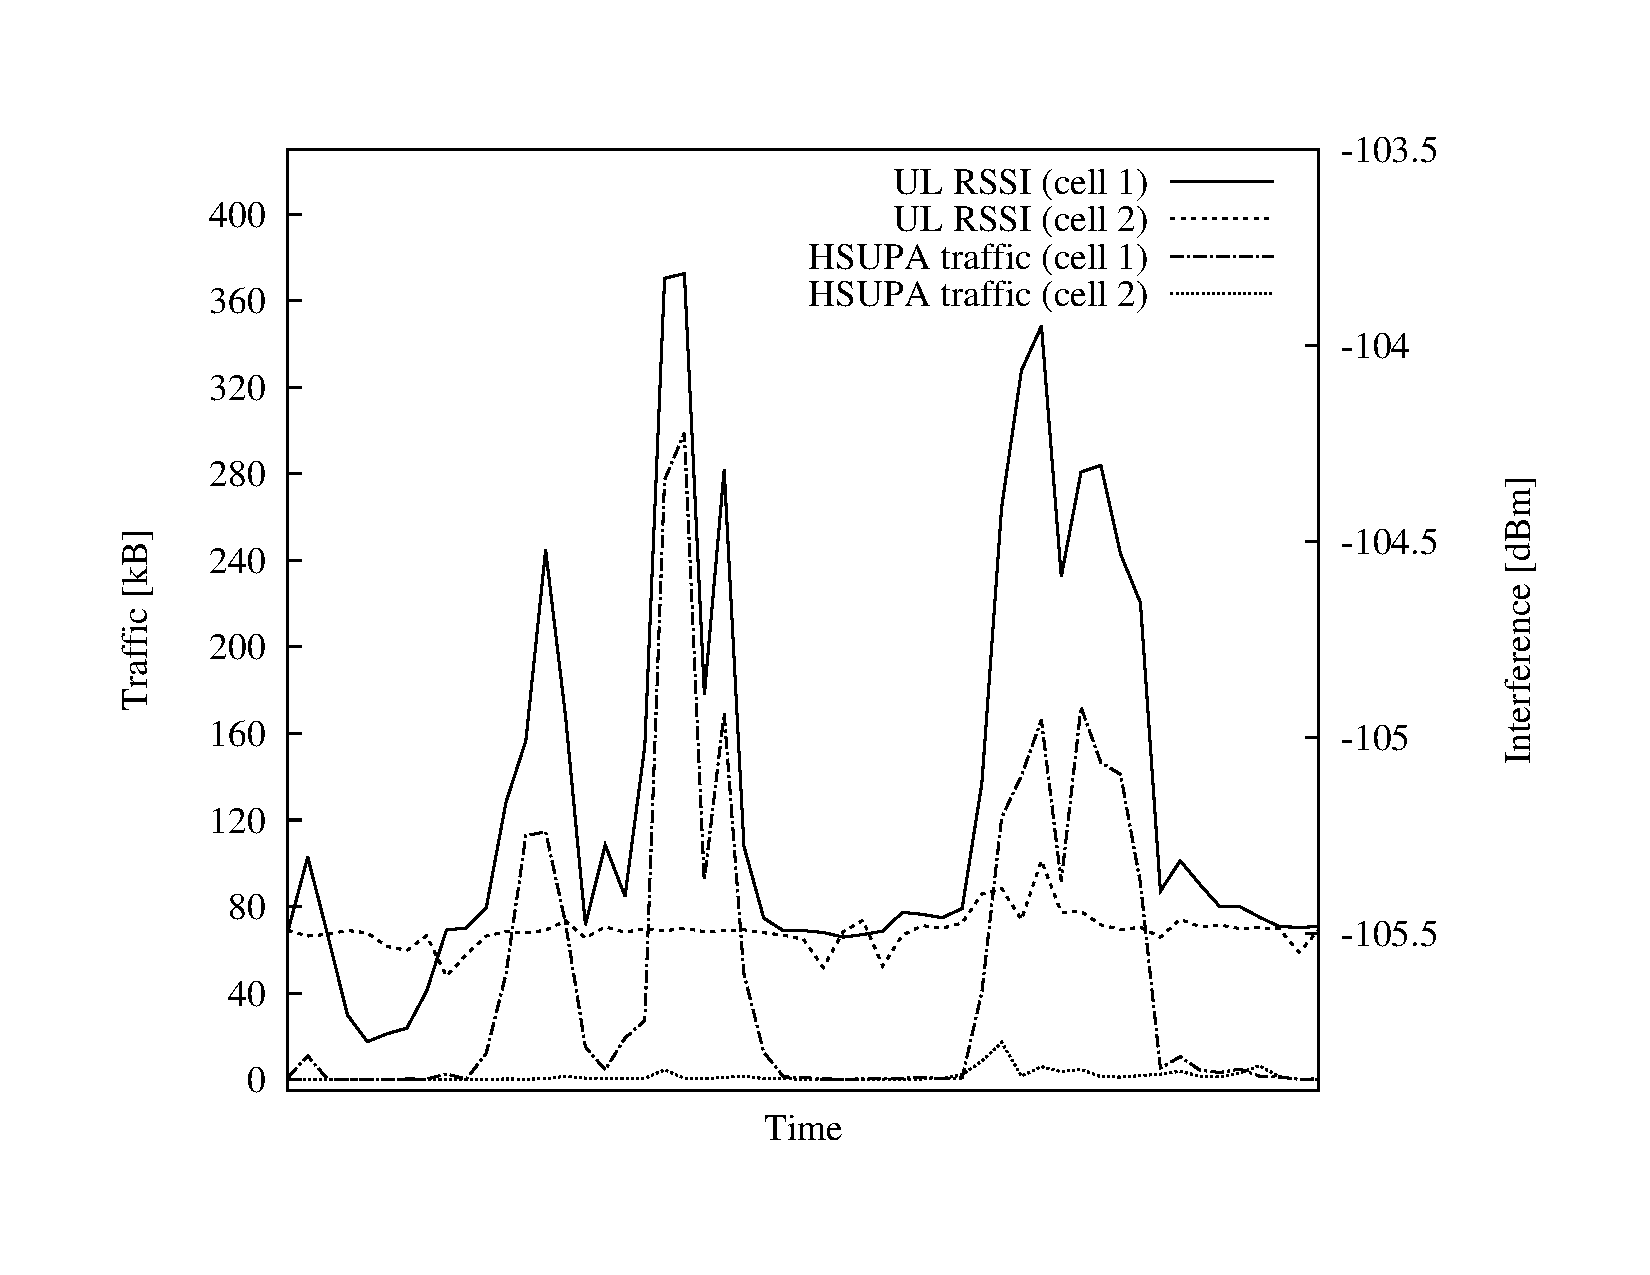
\includegraphics[width=0.9\textwidth]{07-experimental_evaluation-sho_balancing/img/network_normal}\\\vskip -0.3in(a)

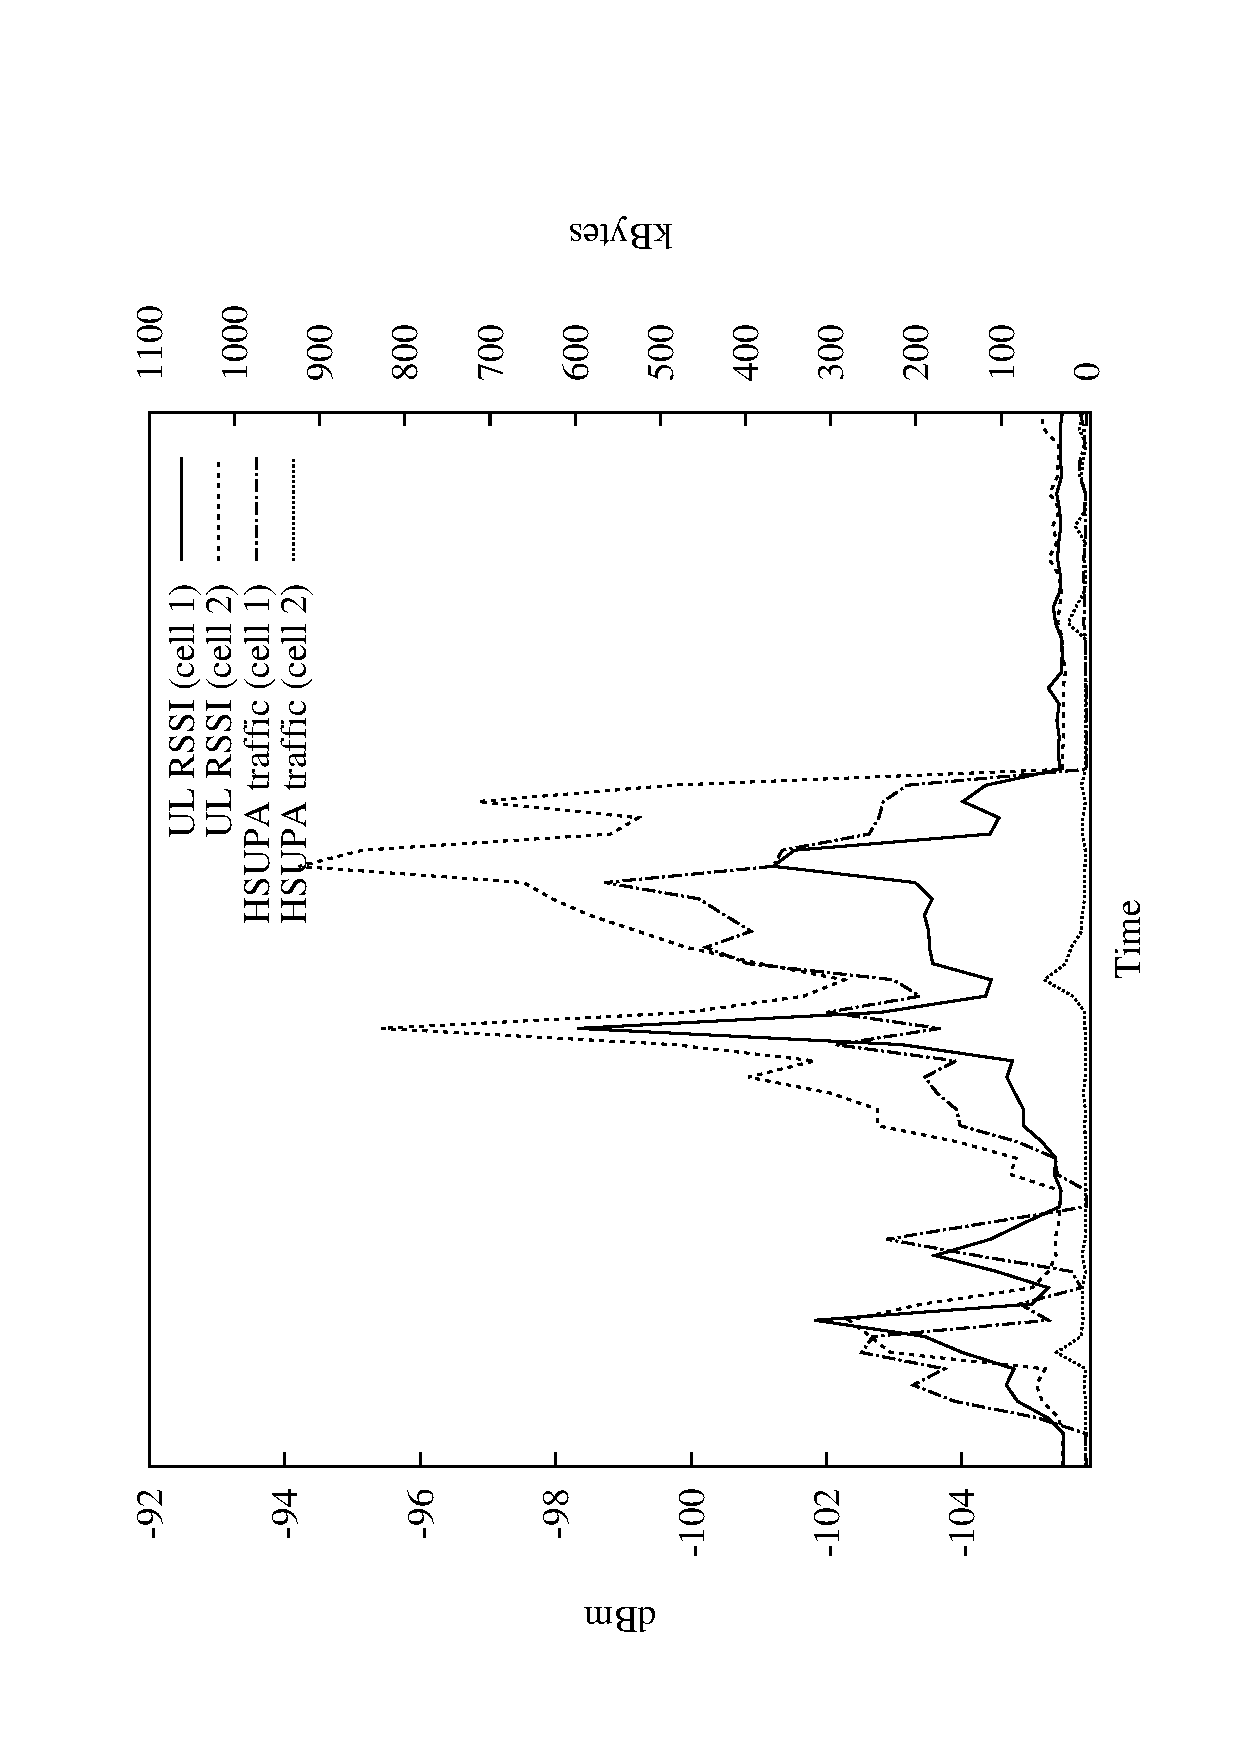
\includegraphics[width=0.9\textwidth]{07-experimental_evaluation-sho_balancing/img/network_problem}\\\vskip -0.3in(b)

\caption{HSUPA traffic and uplink interference with: (a) balanced downlink
and uplink SHO conditions, and (b) unbalanced downlink and uplink
SHO conditions.\label{fig:07-Problem_illustration}}
\end{figure}


Despite several built-in mechanisms, that allow a radio network to
overcome different problems due to the lack of SHO during a HSDPA
connection, some abnormal cases do arise, especially in those areas
where there is SHO capability in the uplink, but none in the downlink.
An example of such a case is depicted in Figure \ref{fig:07-Problem_illustration},
which shows the interference behavior during a HSPA connection in:
(a) normal SHO conditions, and (b) unbalanced SHO conditions. The
plotted data are actual radio network statistics, taken from the mobile
network deployed in Slovenia by Telekom Slovenije, d.d. The graph
on the left, (a), shows a normal HSUPA-enabled service situation,
in which the measured interference is proportional to the traffic
being served. Note how the noise rises with the increased traffic
on cell~1, while its neighbor (cell~2) has almost no interference
nor traffic. Moreover, the graph profile for both traffic and noise
of cell~1 are almost identical. The graph on the right, (b), depicts
a problematic situation, where the noise level does not only rise
on the cell serving the HSUPA services (cell~1), but also on the
neighboring one. Notice how the interference level rises on the cell
that has almost no traffic (cell~2). It is clear that the source
of this noise rise is generated by the active connection on cell~1,
which shows an increase in HSUPA traffic. However, the noise-level
profile on cell~2 does not follow its traffic, as it did in the normal
situation (a). This is due to cell~2 not being part of the active
set. Such situations appear when the UL coverage is larger than the
DL coverage. Interestingly enough, this seems to be an exceptional
case, as Holma and Toskala write in~\cite{holma2006hsdpa}, when
describing the SHO in chapter 5:

''... There is no obvious reason why the serving E-DCH cell would
not be the same as the serving HSDPA cell, and this is also required
to be the case in the specifications.''

Given the described context, the challenge is to achieve the correct
balance or distribution of downlink and uplink SHO areas within a
working UMTS network. Therefore, the network has to be fine-tuned
to improve the SHO-area balancing, thus to avoid the exceptional appearance
of problematic situations, as shown in Figure~\ref{fig:07-Problem_illustration}.
This clearly implies that the mobile network configuration should
not be excessively altered, since other aspects of the network are
working well before starting the optimization process. Hence, the
objective of the optimization problem is to find a pilot-power configuration
for all the cells in the target network, such that the balance of
downlink and uplink SHO areas is improved and other network aspects
are preserved. The optimization process takes into account different
kinds of hardware, e.g., amplifiers, cables, and antennas, adjusting
the pilot powers of the cells.

\bigskip{}


PRATO, as defined in Chapter~\ref{chap:04-Framework-design-and-implementation},
is used as the evaluation framework of the SHO-balancing problem.
A state-of-the-art mathematical model~\cite{nawrocki2006understanding}
describes the downlink and uplink SHO areas. By introducing a penalty-based
objective function and some hard constraints, a formal definition
of the SHO-balancing problem in UMTS networks is given. The mathematical
model and the penalty scores of the objective function are set according
to the configuration and layout of a real mobile network, deployed
in Slovenia by Telekom Slovenije, d.d. The SHO settings are also taken
from the actual network configuration, still they were adapted to
closely model interference and other dynamic aspects of the network.




\section{Related work \label{sec:07-Related-work}}

The SHO optimization has received quite some attention from the scientific
community during the past years. This mainly relates to the importance
it has within the deployed networks that provide high-speed services,
such as video telephony~\cite{chen2010_impact_of_soft_handover}
and data services by means of HSPA \cite{chen2011_coverage_planning_for_optimizing_HSDPA,chen2008cpich}.

Some authors tackled optimization problems at the planning stage of
the network~\cite{Eisenblatter_OptimizationMethodsForUMTSRadioNetworkPlanning,ghosh2011_optimising_CDMA_cell_planning},
considering, among other variables, BS locations and hardware. However,
most mobile operators are unable to apply such methods to a live network,
since the planning phase of the new installation has long been concluded.
Moreover, the great majority of the BSs has already been deployed
and their hardware also installed. Therefore, from the mobile operator's
point of view, mainly parameter and software optimization are the
only tools available, when it comes to QoS improvement (see Chapter~\ref{chap:02-Optimization_of_radio_networks})
and network troubleshooting in the short term.

Optimizing SHO by means of pilot-power adjustment is an established
way of enhancing network capacity, when high-speed services like HSDPA
and HSUPA coexist with legacy technologies~\cite{chen2008cpich}.
In the UMTS, the pilot power is typically between 5\% to 10\% of the
total downlink transmit power of the BS~\cite{RadioNetworkPlanningAndOptimisationForUMTS},
but there is no standardized method to fi{}nd a pilot-power setting.
A number of existing approaches to resolve this issue exist in the
related literature~\cite{WCDMAforUMTS_RadioAccessForThirdGenerationMobileCommunications,Siomina_PilotPowerManagementInWCDMANetworksCoverageControlWithRespectToTrafficDistribution,Ying_CPICHPowerSettingsInIrregularWCDMAMacroCellularNetworks},
being those based on optimization methods the most eff{}ective ones~\cite{Eisenblatter_OptimizationMethodsForUMTSRadioNetworkPlanning,GarciaLozano_CPICHPowerOptimisationByMeansOfSimulatedAnnealingInAnUTRAFDDEnvironment,RadioNetworkPlanningAndOptimisationForUMTS,UMTSRadioNetworkPlanning_OptimizationAndQoSManagementForPracticalEngineeringTasks,siomina2008minimum}.
Such a wide spectrum of available procedures is directly related to
the diverse criteria taken into account when assigning the pilot power
of a cell. The fundamental reason behind this fact is that the pilot
power is a common adjustment vairble of various optimization problems
in radio networks. This is especially true for UMTS networks, due
to their frequency-reuse factor of 1~\cite{WCDMAforUMTS_RadioAccessForThirdGenerationMobileCommunications}.


\section{Radio-network model \label{sec:07-Radio_network_model}}

This section extends the representation of the radio-network model,
previously introduced in Section~\ref{sec:06-Radio_network_model},
Chapter~\ref{chap:06-Experimental-evaluation-the-service-coverage-problem},
in order to include the SHO functionality. In this context, the mathematical
model links the SHO settings with the pilot-power level of each cell,
the best-server pattern, and the network coverage.

By introducing a change step of 0.01~dB and bounding the pilot power
of a cell $c$, $c\in C$, to $\pm2$~dB (relative to the pilot-power
setting the cell had before optimization), the number of elements
in the set $P_{c}$ is reduced. The purpose of this reduction is twofold.
First, since the optimization targets a live network, there is no
need for the algorithms to create complete new configurations, but
just to fine-tune existing ones. Second, the problem complexity is
lowered, because the size of the search space is smaller and discrete.


\subsection{Soft-handover areas \label{sub:07-SHO_areas}}

To obtain a realistic outline of the areas where an UE may potentially
maintain connections to more than one cell, a static version of the
active set, as defined in \cite{nawrocki2006understanding}, is used.
To this end, a SHO window, $\gamma^{\mathrm{sho}}$\nomenclature[S]{$\gamma^{\mathrm{sho}}$}{SHO window.},
and a \textit{\emph{maximum}} active-set size, $as^{\mathrm{max}}$\nomenclature[S]{$as^{\mathrm{max}}$}{Maximum number of neighbouring cells in the active set.},
are introduced. Both parameters are taken from the working configuration
of the real network. It follows that the cells to which an UE $m$,
$m\in M$, may maintain concurrent downlink connections are part of
the set:

\begin{eqnarray}
SHO_{m}^{\downarrow} & = & \left\{ c\vert L_{c^{*}m}^{\downarrow}p_{c^{*}}-L_{cm}^{\downarrow}p_{c}\le\gamma^{\mathrm{sho}}\right\} ,\label{eq:sho_dl}\\
\vert SHO_{m}^{\downarrow}\vert & \le & as^{\mathrm{max}},\nonumber 
\end{eqnarray}


\nomenclature[S]{$SHO_{m}^{\downarrow}$}{Cell set to which a mobile may maintain concurrent downlink connections, i.e. downlink SHO.}

\noindent where $L_{c^{*}m}^{\downarrow}$ is the downlink attenuation
factor of the best-serving cell, and $p_{c^{*}}$ is its pilot power.
Since the number of elements in $SHO_{m}^{\downarrow}$ is at most
$as^{\mathrm{max}}$, the weakest links are removed if there are several
present. This method is well suited for configurations with no hysteresis,
since dynamic effects are ignored in static models \cite{nawrocki2006understanding}. 

Additionally, in the uplink, the set of cells to which an UE can potentially
be in SHO is defined as:

\begin{equation}
SHO_{m}^{\uparrow}=\left\{ c\vert L_{mc}^{\uparrow}p_{m}^{\uparrow}\ge3.16227766\cdot10^{-12}mW\right\} ,
\end{equation}


\nomenclature[S]{$SHO_{m}^{\uparrow}$}{Cell set to which a mobile may maintain concurrent uplink connections, i.e. uplink SHO.}

\noindent where $L_{mc}^{\uparrow}$ is the uplink attenuation factor
from an UE $m$ to a cell $c$, and $p_{m}^{\uparrow}$\nomenclature[S]{$p_{m}^{\uparrow}$}{Uplink transmit power of mobile $m\in M$.}
is the uplink transmit power of $m$.

The static nature of the model intentionally neglects mobility and
dynamic interference by narrowing $\gamma^{\mathrm{sho}}$ down to
2~dB~\cite{nawrocki2006understanding}.


\section{Problem definition \label{sec:07-Problem_definition}}

Using the elements defined in Section~\ref{sec:07-Radio_network_model},
an objective function was formulated in cooperation with a team of
radio engineers of the Radio Network Department at Telekom Slovenije,
d.d. The objective function is constructed as a weighted sum, containing
different costs that penalize the occurrence of specific SHO conditions
in downlink and uplink, which may potentially cause the afore-mentioned
malfunctioning, introduced in Section \ref{sec:07-Motivation}.

A cost-based objective function is the most natural and straight-forward
way of defining the optimization objective. Besides it is easily extendable
to include other future situations, also defining the mutual importance
of the different phenomena taken into account at the optimization
phase.

Hence, the definition of the objective function for the SHO-balancing
problem is the minimization of the sum of penalty scores given as:

\begin{equation}
\min f_{\mathrm{sho}}=\sum_{c\in C}\sum_{m\in M}pf_{\mathrm{cov}}(1-cov_{cm})+pf_{\mathrm{sho}}^{\uparrow}sho_{cm}^{\uparrow}(1-sho_{cm}^{\downarrow})+pf_{\mathrm{sho}}^{\downarrow}sho_{cm}^{\downarrow}(1-sho_{cm}^{\uparrow}),\label{eq:07-objective_function}
\end{equation}


\nomenclature[S]{$f_{\mathrm{sho}}$}{Objective function of the SHO-balancing problem.}

\noindent where 

\begin{equation}
sho_{cm}^{\downarrow}=\begin{cases}
1 & c\in SHO_{m}^{\downarrow}\\
0 & otherwise
\end{cases},
\end{equation}


\begin{equation}
sho_{cm}^{\uparrow}=\begin{cases}
1 & c\in SHO_{m}^{\uparrow}\\
0 & otherwise
\end{cases},
\end{equation}


\noindent and
\begin{itemize}
\item $pf_{\mathrm{cov}}$ represents the penalty factor for uncovered areas,
\item $pf_{\mathrm{sho}}^{\uparrow}$ represents the penalty factor for
uplink SHO areas where SHO is not possible in the downlink, and
\item $pf_{\mathrm{sho}}^{\downarrow}$ represents the penalty factor for
downlink SHO areas where SHO is not possible in the uplink.
\end{itemize}
\bigskip{}


After extensive experimentation, and working in cooperation with the
radio engineers from the Radio Network Department at Telekom Slovenije,
d.d., the penalty factors from Equation~(\ref{eq:07-objective_function})
are set to the following values:
\begin{itemize}
\item $pf_{\mathrm{cov}}=15$,
\item $pf_{\mathrm{sho}}^{\uparrow}=13$, and
\item $pf_{\mathrm{sho}}^{\downarrow}=3$.
\end{itemize}
It is clear that the coverage is the most important quality aspect
from the network point of view (penalty factor $pf_{\mathrm{cov}}$).
Moreover, it imposes the biggest constraint to the optimization process,
since the balance between SHO areas should not sacrifice network coverage.
Another important characteristic that emerges from these values is
the preference for minimizing areas where SHO capability is available
in the uplink, but not in the downlink (penalty factor $pf_{\mathrm{sho}}^{\uparrow}$).
As it has been described in Section~\ref{sec:07-Motivation}, the
consequences of such SHO arrangement produce severe interference in
neighboring cells (Figure~\ref{fig:07-Problem_illustration}), which
may also result in service inaccessibility. The last factor $pf_{\mathrm{sho}}^{\downarrow}$
imposes a penalty value over areas where the SHO capability is available
in the downlink, but not in the uplink. Recall that when accessing
HSPA services, SHO is available only in the uplink. For this reason,
the link throughput may benefit from the SHO in the uplink if it is
available. The relative lower importance of the last penalty factor,
when compared to the other ones, is directly related to the consequences
of the unbalancing that such SHO areas may have on the network. In
this case, only the HSPA throughput is affected, while the service
accessibility should not be an issue, given there is enough uplink
coverage~\cite{holma2006hsdpa}.


\section{Optimization approaches \label{sec:07-Optimization_algorithms}}

The SHO-balancing problem has been tackled using three fundamentally
different optimization algorithms, namely:
\begin{itemize}
\item DE (see Section~\ref{sub:02-DE}, Chapter~\ref{chap:02-Optimization_models}),
from the family of evolutionary algorithms;
\item DASA (see Section~\ref{sub:02-DASA}, Chapter~\ref{chap:02-Optimization_models}),
from the family of swarm-intelligence algorithms; and
\item SA (see Section~\ref{sub:02-SA}, Chapter~\ref{chap:02-Optimization_models}),
from the group of classic metaheuristic algorithms, targeted at combinatorial
optimization problems.
\end{itemize}
Each of these algorithms shall minimize the objective function value
by adopting essentially disparate approaches, hence the diversity
of applying algorithms belonging to different families to solve the
same optimization problem. Therefore, the result analysis shall establish
which of the presented approaches is better suited for solving the
SHO-balancing problem.

The following sections describe how the SHO-balancing problem is represented
by the internal structure of each of the selected algorithms and their
controlling parameters.


\subsection{Differential evolution}

The DE algorithm features a parallel direct search method, which utilizes
a population of $D$-dimensional parameter vectors. The SHO-balancing
problem is expressed in each component of a vector $X$ of the population,
which represents the pilot power of a target cell, i.e.:

\begin{equation}
X_{aG}=\left\{ x_{1},x_{2},\ldots x_{c},\ldots,x_{D}\right\} ,\label{eq:07-DE_mapping}
\end{equation}
where $x_{c}\in P_{c}$ represents a candidate pilot-power setting
of cell $c$, and $G$ indicates the generation of an individual $a$
in the population. Since there are $|C|$ cells in a mobile network,
it follows that the population size, $D=|C|$.

From the different variants of DE, the most popular one is used here,
called \emph{DE/rand/1/bin}. The nomenclature used to name this variant
indicates the way the algorithm works:
\begin{itemize}
\item \emph{DE }denotes the differential evolution algorithm,
\item \emph{rand }indicates that the individuals selected to compute the
mutation values are randomly chosen,
\item 1\emph{ }specifies the number of pairs of selected solutions used
to calculate the crossover vector, and
\item \emph{bin }means that a binomial recombination operator is used.
\end{itemize}

\subsection{Differential ant-stigmergy algorithm}

The mapping between the balancing problem and DASA is similar to the
one for DE:

\begin{equation}
X_{a}=\left\{ x_{1},x_{2},\ldots x_{i},\ldots,x_{D}\right\} \label{eq:07-DASA_mapping}
\end{equation}


\noindent In this case, each ant, $a$, creates its own solution vector,
$X_{a}$, during the minimization process. At the end of every iteration,
and after all the ants have created solutions, they are evaluated
to establish if any of them is better than the best solution found
so far.


\subsection{Simulated annealing}

From the SA perspective, the system under optimization is in a given
\emph{state} at each time step during the process. The objective function
maps a system state to a value known as the \emph{energy} of the system
in that state. A \emph{move} in the search space represents a change
in the state of the system. After making a move, the system may exhibit
lower or higher energy, depending on the results of the objective
function.

Algorithm~\ref{alg:07-SA_move} shows the pseudo-code of a move in
the search space of possible pilot-power settings, resulting in a
new state of the system.

\begin{algorithm}
\centering

\caption{A move in the search space of SA for solving the SHO-balancing problem.\label{alg:07-SA_move}}


\begin{algorithmic}
\State $\mathbf{c'} \gets pick\_random\_cell(C)$
\Repeat
	\If{$ \mathrm{uniform}[0,1] < 0.5$}
		\State $p_{c'}^{\mathrm{new}} \gets p_{c'}+0.01$
	\Else
		\State $p_{c'}^{\mathrm{new}} \gets p_{c'}-0.01$
	\EndIf
\Until{$p_{c'}^{\mathrm{new}}\in P_{c'}$}
\State $p_{c'} \gets p_{c'}^{\mathrm{new}}$
\end{algorithmic}
\end{algorithm}


At the first step, a cell, $c'$, is randomly selected from the set
of all cells in the network, $C$. In step 2, a change of +0.01~dB
or -0.01~dB is applied with 50\% probability to $p_{c'}$. The pilot
power of cell $c'$ is expressed in dBm. The randomly generated pilot-power
setting, $p_{c'}^{\mathrm{new}}$, is checked for validity in step
3, i.e., it must be an element of the set $P_{c'}$. If $p_{c'}^{\mathrm{new}}$
is not a valid pilot power, step 2 is executed again, generating another
random pilot power. Finally, in step 4, the pilot power of cell $c$
is replaced by $p_{c'}^{\mathrm{new}}$.

It is important to note that, as long as $|P_{c'}|>1$, the pseudo-code
shown in Algorithm~\ref{alg:07-SA_move} shall never be trapped in
an endless loop. On the other hand, if $|P_{c'}|<2$, there are no
candidate pilot powers for cell $c'$, and thus there is no possibility
of optimization. Notice also that the acceptance of a move in the
search space is left to SA and its stochastic components.


\section{Simulations \label{sec:07-Simulations}}

The simulations were performed over the target geographical area,
for which DEM and clutter data were available. The mobile users were
assumed to be uniformly distributed. The SHO conditions were determined
by the relative received-signal quality from different cells, and
the SHO window, which triggers the addition of a cell to a user's
active set~\cite{WCDMAforUMTS_RadioAccessForThirdGenerationMobileCommunications}.


\subsection{Test network}

The test network used for the simulations, Net$_{7}$, is a subset
of the real UMTS network deployed in Slovenia by Telekom Slovenije,
d.d. It represents a network extending over a hilly terrain, combining
both rural and middle-dense suburban areas, which contains 25 cells
within an area of more than 150~km$^{2}$. Table~\ref{tab:07-Test_network_properties}
shows some characteristics of the test network used, and Figure~\ref{fig:07-Coverage_areas}
shows the area under radio coverage, $A_{\mathrm{covered}}$, within
$A_{\mathrm{total}}$.

\begin{table}[h]
\caption{Technical characteristics of Net$_{7}$, the test network used for
the SHO-balancing problem. \label{tab:07-Test_network_properties}}


\centering

\begin{tabular}{cc}
\hline 
Number of cells & $25$\tabularnewline
Coverage threshold (RSCP) & $-115$~dBm\tabularnewline
SHO window ($\gamma^{\mathrm{sho}}$) & $2$~dB\tabularnewline
User equipment ($p_{m}^{\uparrow}$) & $21$~dBm, power class 4\tabularnewline
Pixel resolution & $25$~m$^{2}$\tabularnewline
Population density & $398$/km$^{2}$\tabularnewline
\hline 
\end{tabular}
\end{table}


\begin{figure}
\centering

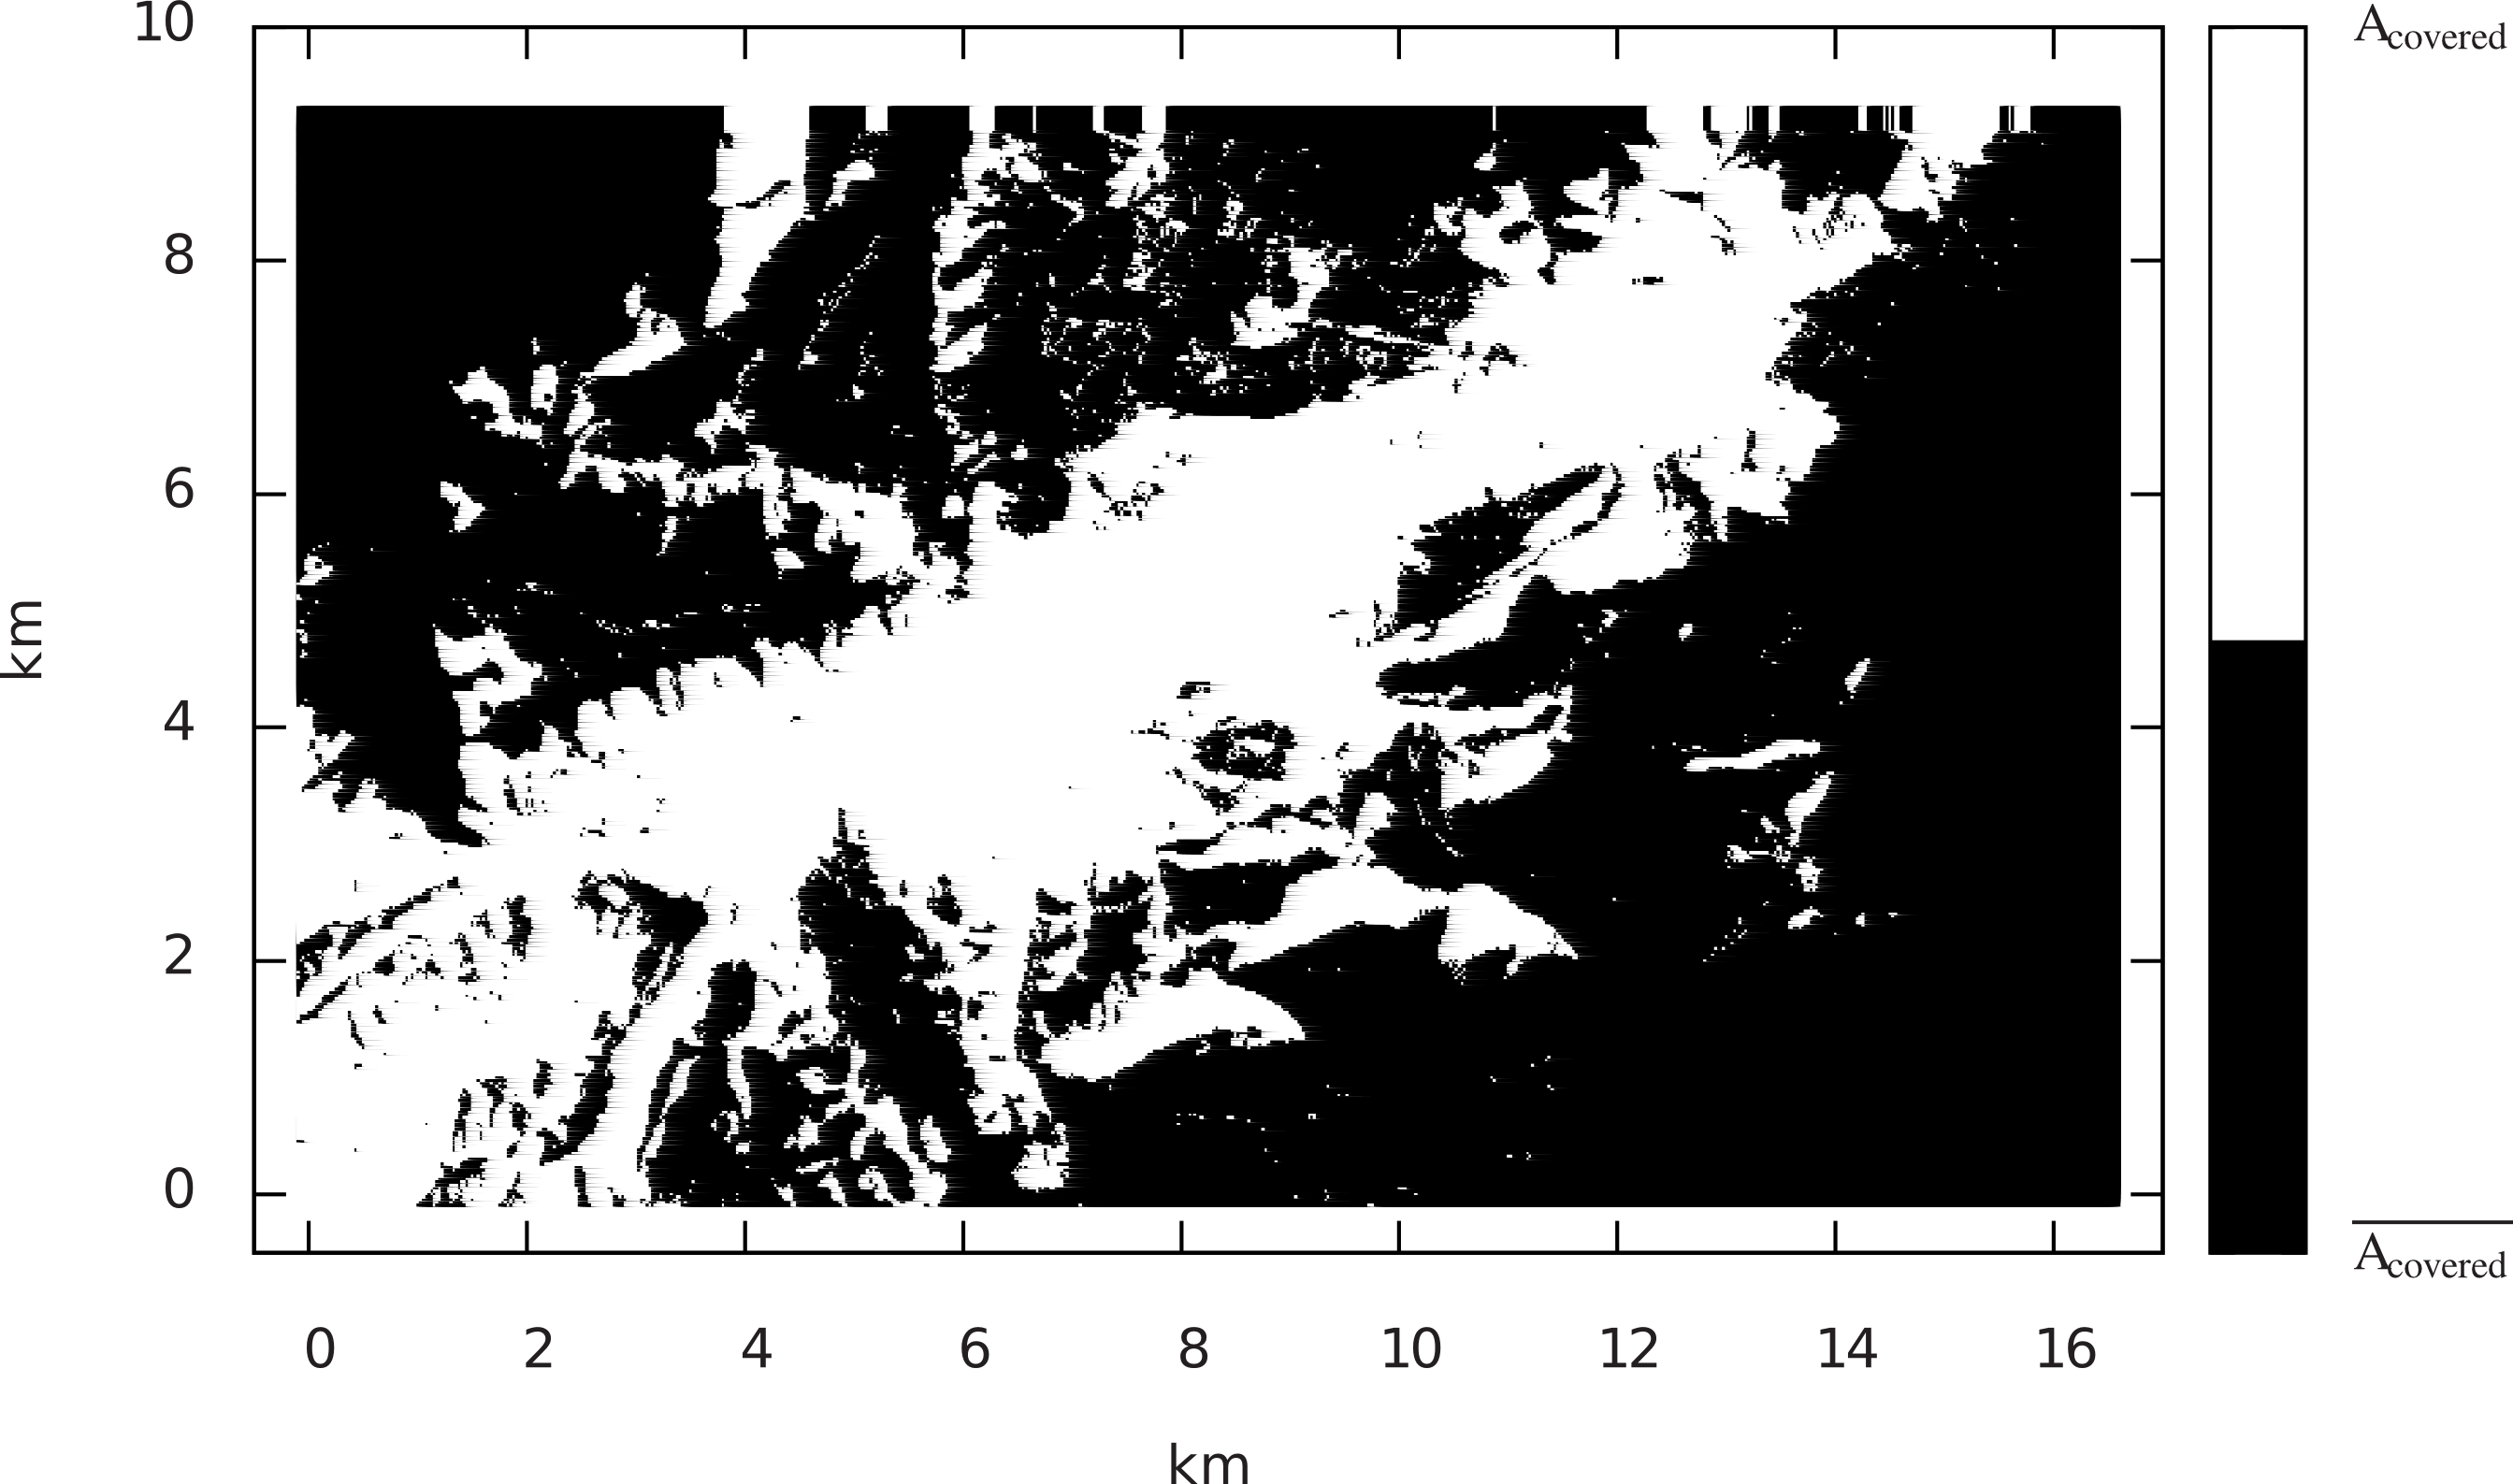
\includegraphics[width=1\textwidth]{07-experimental_evaluation-sho_balancing/img/coverage_area}

\caption{Area under radio coverage, $A_{\mathrm{covered}}$, and without radio
coverage, $\overline{A_{\mathrm{covered}}}$, within the complete
geographical area, $A_{\mathrm{total}}$, of test network Net$_{7}$.\label{fig:07-Coverage_areas}}
\end{figure}



\subsection{Algorithm parameters}

In this section, the algorithm-parameter setup used during the simulations
is given. In all three cases, the parameter names are given with their
respective values and descriptions.

The parameters controlling the behavior of the DE algorithm were set
as follows:
\begin{itemize}
\item $NP=100$, the population size;
\item $G_{max}=1000$, the maximum number of generations for the algorithm
to run;
\item $CR=0.8$, the crossover constant; and
\item $F=0.5$, the mutation-scaling factor.
\end{itemize}
As for DASA, the parameters were set to the following values:
\begin{itemize}
\item $m=10$, the number of ants;
\item $b=10,$ the discrete base;
\item $q=0.2$, the pheromone dispersion factor;
\item $s_{+}=0.01$, the global scale-increasing factor;
\item $s_{-}=0.01$, the global scale-decreasing factor; and 
\item $e=1.0^{-2}$, the maximum parameter precision.
\end{itemize}
There are only two parameters controlling SA, namely:
\begin{itemize}
\item $t_{initial}=125$, the initial temperature; and
\item $it=100,000$, the total number of iterations.
\end{itemize}
In this case, the exponential-lowering schema was chosen as the way
the temperature was lowered during the SA searches.


\subsection{Experimental environment}

All experiments were carried out on a 4-core Intel i7 2.67~GHz desktop
computer with 6~GB of RAM running a 64-bit Linux operating system.
The implementation languages used were C and Python, with the latter
mostly used as \textquoteleft{}glue\textquoteright{} to hold the different
implementation parts together, as well as for I/O operations. To lower
the time needed to run one optimization round, the entire objective-function
evaluation was implemented using OpenCL and executed on a nVidia GeForce
GTX 260. This individual change exhibited more than 15-fold, execution-time
speedup, when compared to the original CPU-only version.


\subsection{Results \label{sub:07-Results}}

In this section, the performance of the selected algorithms is presented.
The analysis includes aspects related to solution quality and convergence
speed. All experimental results were obtained after 30 independent
runs, each of them limited to a maximum of 100,000 evaluations. The
gathered results are shown in Table~\ref{tab:07-Algorithm_performance}.

\begin{table}
\centering

\caption{Solution-quality performance of the three algorithms, after 30 independent
runs\textit{\emph{.}}\textit{\label{tab:07-Algorithm_performance}}}


\begin{tabular}{ccccc}
\toprule 
 & Best & Worst & Mean & Std. deviation\tabularnewline\addlinespace
\midrule
DE & 2,286,292.00 & 2,286,541.00 & 2,286,517.09 & 62.06\tabularnewline
DASA & 2,286,446.00 & 2,286,633.00 & 2,286,592.00 & 26.19\tabularnewline
SA  & 2,293,350.00 & 2,295,570.00 & 2,294,626.50 & 663.75\tabularnewline
\bottomrule
\end{tabular}
\end{table}


It may be observed that DE reached the lowest objective-function value,
closely followed by DASA. Likewise, both algorithms arrived at very
similar results for the worst, mean and standard-deviation values.
SA, on the other hand, did not achieve comparable values, since its
results are behind those of DE and DASA. Notice that even the best
SA solution is no better than the worst solution of DASA. Moreover,
the standard deviation exhibited by SA is one order of magnitude bigger
than those of DASA and DE.

\begin{figure}
\centering

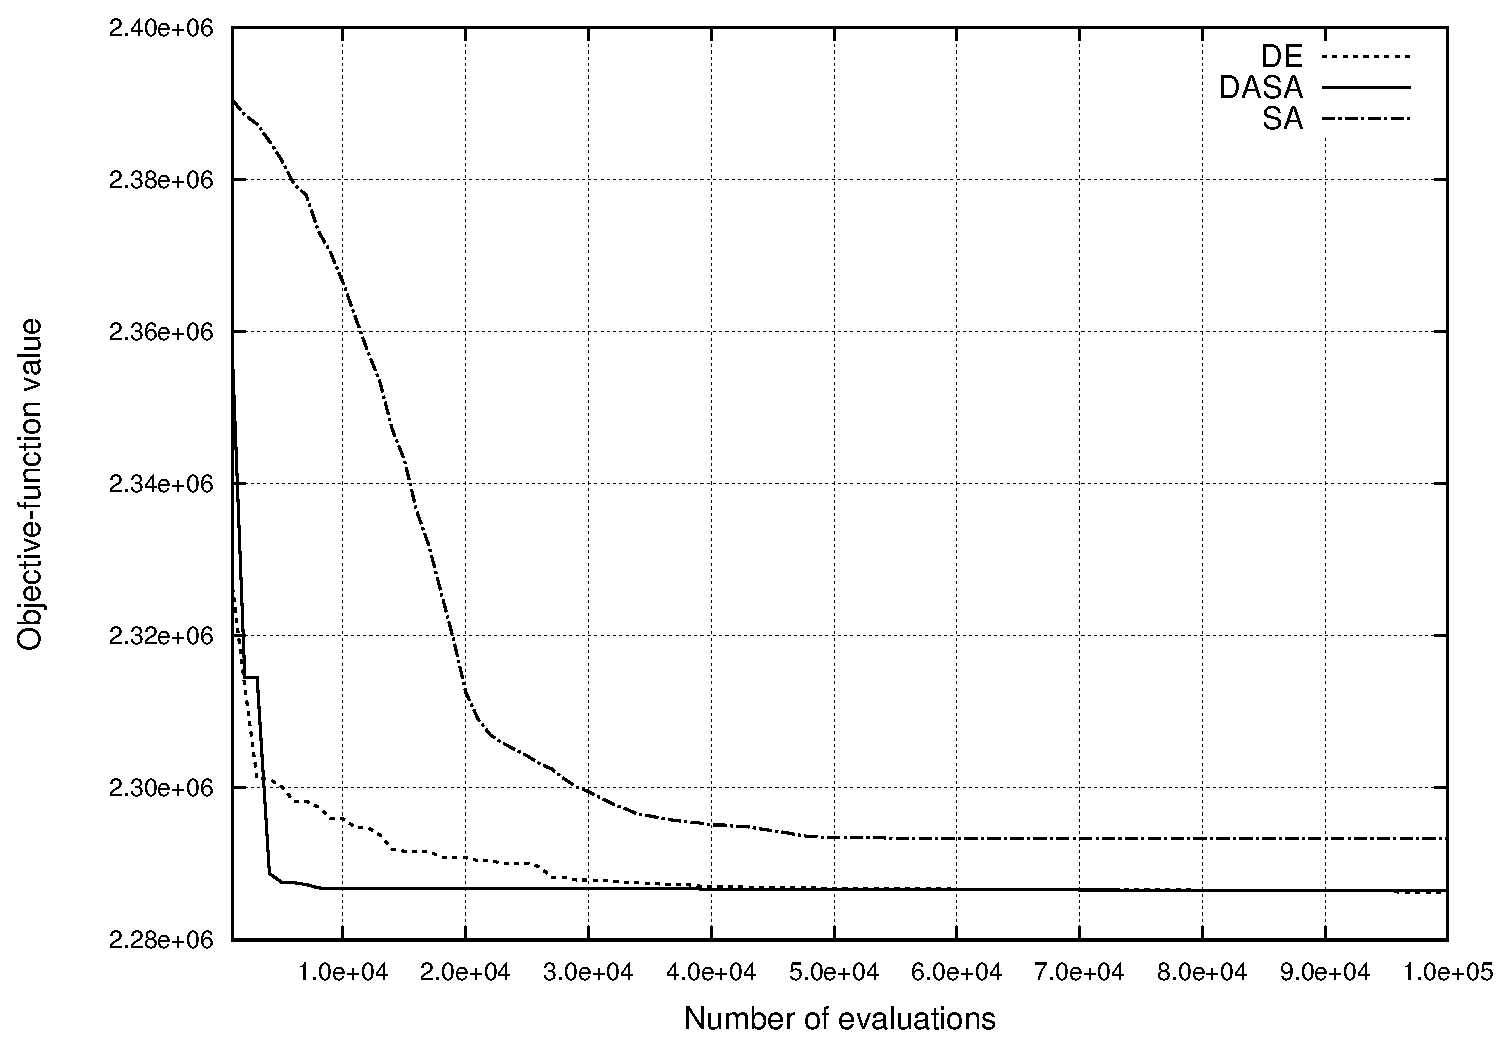
\includegraphics[width=0.9\textwidth]{07-experimental_evaluation-sho_balancing/img/algorithm_convergence}

\caption{Convergence analysis for each of the three algorithms, i.e., DE, DASA
and SA, showing the best results obtained for the SHO-balancing problem.\label{fig:07-Algorithm_convergence}}
\end{figure}


The convergence of the best-recorded run of each of the three algorithms
is shown in Figure~\ref{fig:07-Algorithm_convergence}. It is worth
mentioning that every optimization run starts from a different solution,
randomly constructed by picking a pilot-power setting, $p_{c}^{k}$,
from every $P_{c}$, $1\le k\le|P_{c}|$, $\forall c\in C$. Notice
how fast DASA converged to a good solution. After a number of evaluations
without improvement, DASA resets itself and continues searching from
a new random point within the search space \cite{korosec2010_DASA}.
DE also converged considerably fast, although not as fast as DASA
did. It this case, DE does not reset itself if the current solution
cannot be improved. Despite this, and based on the flat profile the
graph exhibits towards the end of the optimization run, it is clear
that 100,000 evaluations is an adequate stopping criterion for all
algorithms. The third algorithm, SA, slowly converged towards the
best solution found, even though it was not as good as the solutions
found by DE and DASA. 

The three convergence profiles shown in Figure~\ref{fig:07-Algorithm_convergence}
give a clearer notion about the way these algorithms explore the search
space of the SHO-balancing problem.

The simulation-running times have been intentionally omitted, since
the algorithm implementations are fundamentally different and therefore
not comparable with each other.


\subsubsection{Performance analysis}

\begin{table}
\centering

\caption{Improvement analysis of the best solution that each algorithm achieved
for the SHO-balancing problem.\textit{\label{tab:07-Optimization_result_analysis}}}


{\scriptsize{}}%
\begin{tabular}{ccccccc}
\toprule 
 & {\scriptsize{Uncovered}} & {\scriptsize{Covered, no SHO}} & {\scriptsize{SHO}} & {\scriptsize{no SHO$^{\downarrow}$, SHO$^{\uparrow}$}} & {\scriptsize{SHO$^{\downarrow}$, no SHO$^{\uparrow}$}} & {\scriptsize{Total}}\tabularnewline\addlinespace
\midrule
{\scriptsize{Before opt.}} & {\scriptsize{63.00 \%}} & {\scriptsize{15.11 \%}} & {\scriptsize{15.73 \%}} & {\scriptsize{1.80 \%}} & {\scriptsize{4.36 \%}} & {\scriptsize{100.00 \%}}\tabularnewline
\cmidrule{2-7} 
{\scriptsize{DE sol.}} & {\scriptsize{60.23 \%}} & {\scriptsize{16.13 \%}} & {\scriptsize{16.09 \%}} & {\scriptsize{1.47 \%}} & {\scriptsize{6.08 \%}} & {\scriptsize{100.00 \%}}\tabularnewline
{\scriptsize{DASA sol.}} & {\scriptsize{60.24 \%}} & {\scriptsize{16.16 \%}} & {\scriptsize{16.90 \%}} & {\scriptsize{1.46 \%}} & {\scriptsize{5.24 \%}} & {\scriptsize{100.00 \%}}\tabularnewline
{\scriptsize{SA sol.}} & {\scriptsize{60.42 \%}} & {\scriptsize{16.55 \%}} & {\scriptsize{15.97 \%}} & {\scriptsize{1.56 \%}} & {\scriptsize{5.50 \%}} & {\scriptsize{100.00 \%}}\tabularnewline
\cmidrule{2-7} 
{\scriptsize{DE impr.}} & {\scriptsize{+4.40 \%}} & {\scriptsize{+6.75 \%}} & {\scriptsize{+2.29 \%}} & {\scriptsize{+18.33 \%}} & {\scriptsize{-39.45 \%}} & {\scriptsize{---}}\tabularnewline
{\scriptsize{DASA impr.}} & {\scriptsize{+4.38 \%}} & {\scriptsize{+6.95 \%}} & {\scriptsize{+7.44 \%}} & {\scriptsize{+18.88 \%}} & {\scriptsize{-20.18 \%}} & {\scriptsize{---}}\tabularnewline
{\scriptsize{SA impr.}} & {\scriptsize{+4.09 \%}} & {\scriptsize{+9.53 \%}} & {\scriptsize{+1.52 \%}} & {\scriptsize{+13.33 \%}} & {\scriptsize{-26.15 \%}} & {\scriptsize{---}}\tabularnewline
\cmidrule{2-7} 
{\scriptsize{Avg. impr.}} & {\scriptsize{+4.29 \%}} & {\scriptsize{+7.74 \%}} & {\scriptsize{+3.75 \%}} & {\scriptsize{+16.85 \%}} & {\scriptsize{-28.59 \%}} & {\scriptsize{---}}\tabularnewline
\bottomrule
\end{tabular}
\end{table}


Table~\ref{tab:07-Optimization_result_analysis} presents the analysis
of the obtained results from the network point of view. After 30 independent
runs of each of the three algorithms, the best results obtained where
evaluated for the improvement and the decline of each of the measured
network-performance aspects. The results are shown in Table~\ref{tab:07-Optimization_result_analysis},
where '+' indicates improvement and '-' indicates a decline of a given
criteria. Overall, it may be observed that the measured criteria have
been significantly improved. The only exception is the measure for
downlink SHO, without SHO in the uplink (labeled as `SHO$^{\downarrow}$,
no SHO$^{\uparrow}$'), which shows an expected decline, since it
is the optimization aspect with the lowest penalty-factor value.

The coverage has been improved with an average of 4.29\%, whereas
the coverage area where there is no SHO capability, has been increased
7.74\% in average. Areas where SHO is available in both downlink and
uplink have also been improved, i.e., 3.75\% in average. This particular
improvement is interesting from the optimization point of view, because
it had no explicit penalty factor set. Therefore, this may be understood
as a consequence of the correct representation of the different network
aspects in the objective function.

\begin{figure}[H]
\centering

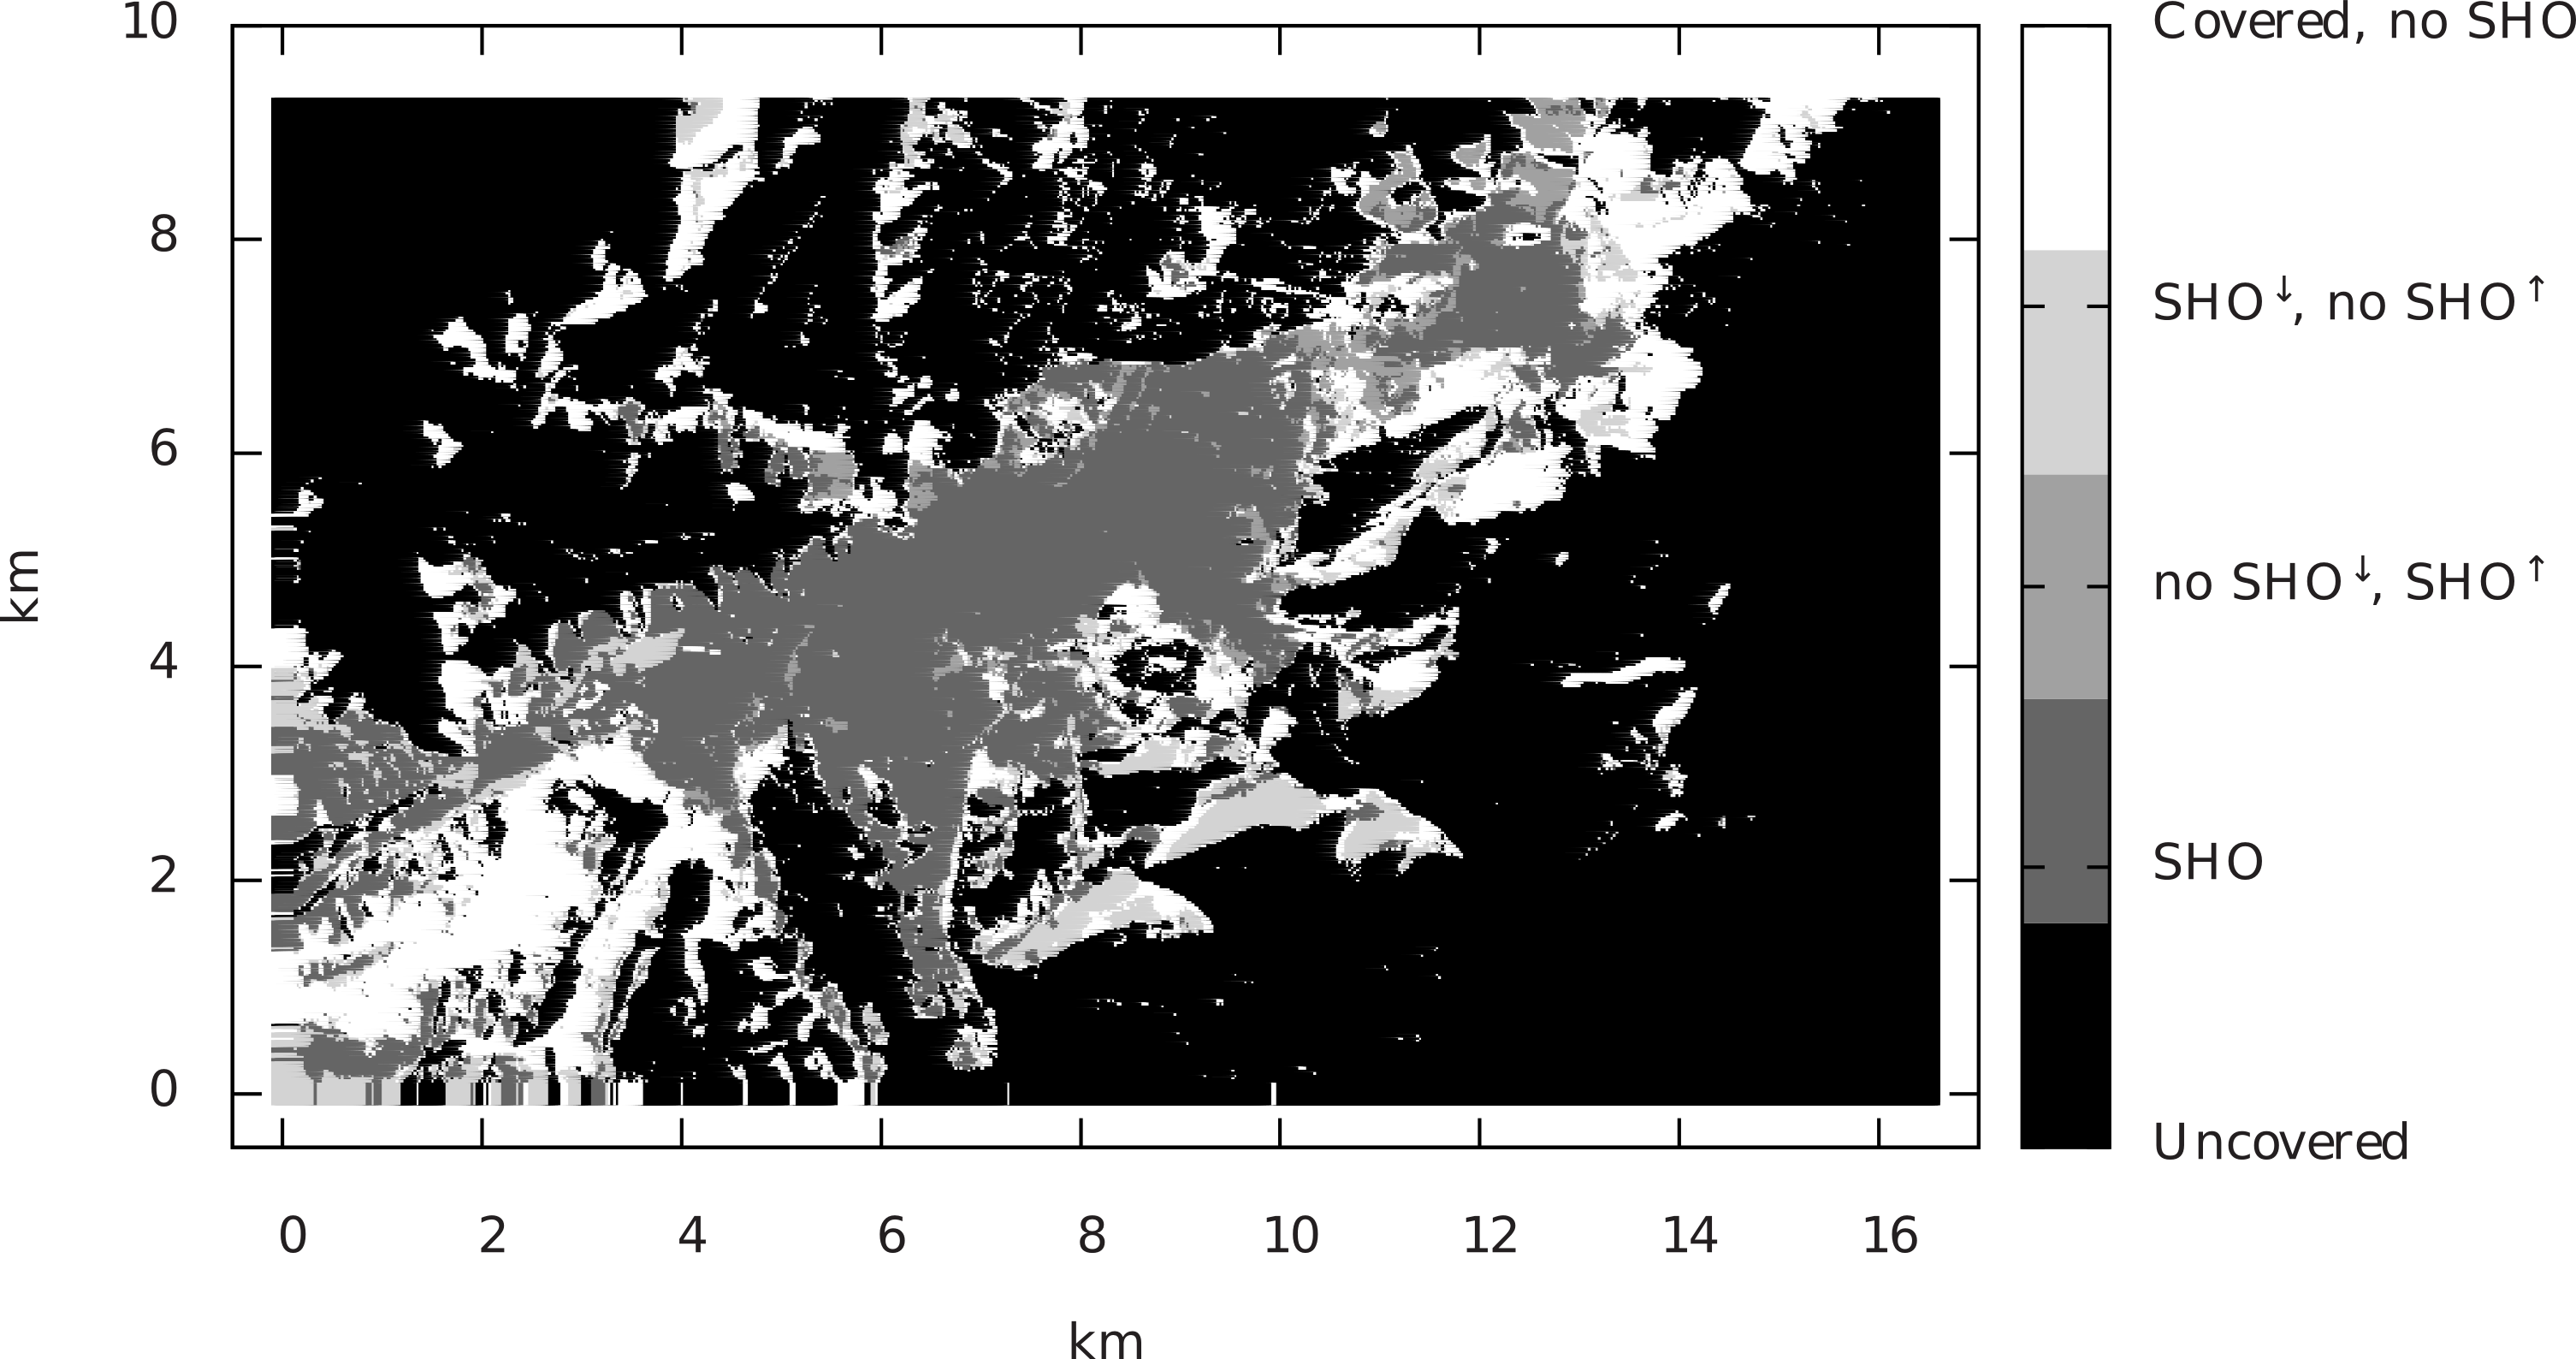
\includegraphics[width=1\textwidth]{07-experimental_evaluation-sho_balancing/img/sho_areas_initial}

\caption{Spatial distribution of the SHO areas before the optimization.\label{fig:07-SHO_areas_initial}}
\end{figure}


\begin{figure}[H]
\centering

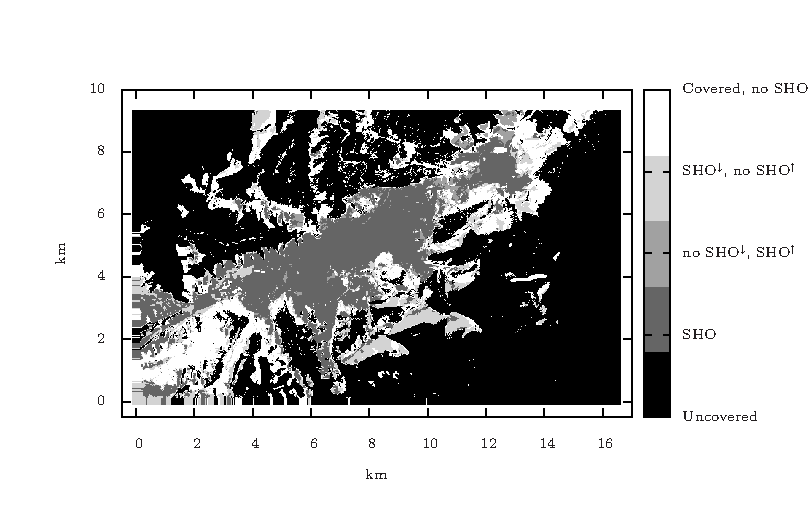
\includegraphics[width=1\textwidth]{07-experimental_evaluation-sho_balancing/img/sho_areas_final}

\caption{Spatial distribution of the SHO areas after the optimization.\label{fig:07-SHO_areas_final}}
\end{figure}


The second most important optimized aspect in the SHO-balancing problem
is the proportion of areas with uplink SHO and no SHO in the downlink
(labeled as `no SHO$^{\downarrow}$, SHO$^{\uparrow}$' in Table~\ref{tab:07-Optimization_result_analysis}).
This particular condition has been improved by almost 17\% in average,
greatly reducing the possibility of interference in neighboring cells
when serving HSPA traffic. The last measured aspect takes into account
areas with downlink SHO and no SHO in the uplink (labeled as `SHO$^{\downarrow}$,
no SHO$^{\uparrow}$' in Table~\ref{tab:07-Optimization_result_analysis}).
This condition, although it hasn't improved, does not expose the mobile
network to malfunctioning, only to reduced throughput within these
specific areas. However, the reduced throughput is relative, since
there are many cells capable of serving HSDPA data access, as the
downlink SHO condition confirms. For this reason, the serving cell
should not only deliver HSDPA, but also take care of the user signaling
and power control, received in the uplink. Clearly, this is only feasible
in areas where uplink coverage is guaranteed.

It is worth mentioning that the simulation results were obtained for
a real radio network with actual configuration data. Moreover, the
hard constraints imposed to the optimization process (the pilot power
limited to the $\pm$2~dB interval) ensure that the resulting configuration
may be immediately applied to a mobile network. This fact can be contrasted
with the spatial distribution of each of the optimized aspects, before
and after applying the optimization results, as it is shown in Figures~\ref{fig:07-SHO_areas_initial}
and~\ref{fig:07-SHO_areas_final}. The lack of any prominent visual
change in Figures~\ref{fig:07-SHO_areas_initial} and~\ref{fig:07-SHO_areas_final}
is a desired consequence of the fine-tuning procedure the network
has been exposed to. Still, the improvements are present precisely
over the areas that are most exposed to malfunctioning due to unbalanced
SHO, e.g., the cell-coverage borders.

\clearpage{}


\section{Summary \label{sec:07-Summary}}

This chapter formally introduced a new optimization problem for 3G
networks: the SHO-balancing problem. A characterization of the consequences
that unbalanced SHO areas have on the quality of HSPA services was
also given. Particularly, tackling the SHO-balancing problem was possible
due to the improved performance delivered by the evaluation framework
PRATO (see Chapter~\ref{chap:04-Framework-design-and-implementation}).

\noindent Using a extension of the radio-network model presented in
Section~\ref{sec:06-Radio_network_model}, Chapter~\ref{chap:06-Experimental-evaluation-the-service-coverage-problem},
the penalty scores of the objective function were set according to
the configuration and layout of a real mobile network, deployed in
Slovenia by Telekom Slovenije, d.d. 

The balancing problem has been tackled by three optimization algorithms,
namely DE, DASA and SA. All three algorithms were able to improve
the given network configuration, being DE the most successful one.
The presented results confirm that a great proportion of the SHO areas,
that were not balanced before the optimization, were corrected, therefore
significantly reducing the possibility of HSPA-service failures. Additionally,
radio coverage was improved, while all other essential network services
were not altered.

One of the key advantages of the presented method is that it targets
the optimization of a deployed network, for which the focus is to
fine-tune the existing configuration instead of creating complete
new solutions. Furthermore, a deployed network has a great number
of hard-constraints that should be taken into account at the optimization
stage. Yet, the presented approach is simple and versatile enough
to be used in practically any working UMTS network. Moreover, the
introduced model is applicable for mobile networks in heterogeneous
environments, because it imposes no restrictions regarding cell layout
or radio-propagation characteristics, which are completely adaptable
through PRATO.

It is important to note that some methods proposed in this chapter
have been particularly designed for problems that emerge during the
planning of 3G radio networks. Despite this, they may be adapted to
other standards, e.g., 2G and 4G, without lose of generality.
